\renewcommand{\nomebreve}{block\_diag\_mat}
\renewcommand{\titolo}{Detecting blocks in a matrix}

\introduzione{}

\sezionetesto{Terminologia di contesto}

\emph{Puoi provare a saltare la lettura di questa sezione. Ci tornerai se ti accorgi che delle nozioni non ti sono chiare.}\\

\noindent
Una matrice di interi è detta \emph{nulla} quando tutti i suoi valori sono nulli. 
Una \emph{matrice diagonale} è una matrice quadrata dove tutti i valori non ricompresi nella diagonale principale sono nulli.
Una \emph{matrice a blocchi} è una matrice di matrici (chiamate `blocchi`) dove tutti i blocchi di una stessa riga (rispettivamente, colonna) hanno lo stesso numero di righe (rispettivamente, colonne).
Una \emph{matrice diagonale a blocchi} è una matrice che possa essere letta come una matrice quadrata di blocchi, dove tutti i blocchi sulla diagonale principale sono matrici quadrate mentre gli altri sono nulli.
Una tale matrice $\mathbf{A}$ ha la seguente forma

\begin{figure}[!h]
\[
\mathbf{A} = \begin{bmatrix} 
  \mathbf{A}_1 & \mathbf{0}    & \cdots & \mathbf{0}   \\
  \mathbf{0}   & \mathbf{A}_2  & \cdots & \mathbf{0}   \\
  \vdots       & \vdots        & \ddots & \vdots       \\
  \mathbf{0}   & \mathbf{0}    & \cdots & \mathbf{A}_n
\end{bmatrix}
\]
  \label{fig:block_structure}
  \caption{lettura strutturale di una matrice diagonale a blocchi come suddivisa nei suoi blocchi}
\end{figure}

dove $\mathbf{A}_k$ è una matrice quadrata per tutti i $k = 1, \ldots, n$.
Se $k$ è il numero dei blocchi principali (quelli sulla diagonale principale), il numero totale di blocchi sarà $k^2$.
La figura potrà chiarire meglio.
\begin{table}[!h]
  \begin{minipage}{.5\textwidth}
    \centering
    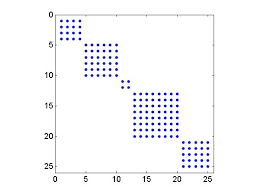
\includegraphics[width=0.60\textwidth]{figures/block_diag_mat_gen_example.png}\\
    {\bf vedi:} struttura di una matrice diagonale a blocchi
  \end{minipage}%
  \begin{minipage}{.5\textwidth}
    \centering
    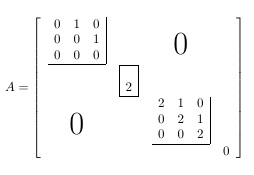
\includegraphics[width=0.60\textwidth]{figures/block_diag_mat_one_example_with_structure_highlighted.png}\\
    {\bf nota:} anche i valori ricompresi nei blocchi della diagonale possono essere nulli
    \end{minipage}
%}      
\end{table}

Anche se i blocchi non-principali possono essere rettangolari, tutti i blocchi principali e quindi anche la matrice stessa sono quadrati.
Di converso, ogni matrice quadrata può essere vista come una matrice diagonale a blocchi di un solo blocco. Tuttavia, la nostra ambizione è quella di individuare una decomposizione in quanti più blocchi possibile, che consenta maggior parallellismo computazionale nelle applicazioni. Una matrice $n\times n$ può essere considerata una matrice a blocchi con $n$ blocchi principali se e solo se è una matrice diagonale. Queste decomposizioni trovano ad esempio motivazione nella formula che dice che il determinante di una matrice a blocchi è dato dal prodotto dei determinanti dei suoi blocchi principali (questo spiega perchè la nozione più diffusa richiede che tutti i blocchi principali siano matrici quadrate). E tale deve quindi essere anche la matrice $\mathbf{A}$ stessa. 

\newpage
\sezionetesto{Il nostro problema}

In questo problema consideriamo quindi anche una nozione più ampia, che rilassa il vincolo che i blocchi sulla diagonale principale debbano essere matrici quadrate. Ciò consente decomposizioni in un numero maggiore di blocchi e al tempo stesso generalizza la decomposizione a tutte le matrici, incluse quelle rettangolari.
La struttura dei blocchi resta una matrice quadrata, e i blocchi non-principali sono tutti ancora matrici nulle, sempre come in Figura~1. Consentiamo però ora ai blocchi principali di essere matrici arbitrarie (anche rettangolari).
Ecco un esempio di come una stessa matrice possa offrire più decomposizioni (ne riportiamo solo 2 delle 8 in totale) di cui quella a destra è quella ottima.

\begin{table}[!h]
  \begin{minipage}{.5\textwidth}
    \centering
\[
\left(
\begin{array}{cccccc|ccccc}
    1 & 0 & 3  & 0 & 0 & 0   &  0 & 0 & 0 & 0  & 0     \\
    0 & 0 & 0  & 2 & 1 & 5   &  0 & 0 & 0 & 0  & 0     \\   \hline
    0 & 0 & 0  & 0 & 0 & 0   &  6 & 0 & 0 & 0  & 0     \\
    0 & 0 & 0  & 0 & 0 & 0   &  7 & 0 & 0 & 0  & 0     \\
    0 & 0 & 0  & 0 & 0 & 0   &  2 & 0 & 5 & 0  & 0     \\
    0 & 0 & 0  & 0 & 0 & 0   &  0 & 0 & 3 & 2  & 0     \\
    0 & 0 & 0  & 0 & 0 & 0   &  0 & 0 & 0 & 0  & 2     \\
\end{array}\right)
\]
    {\bf sub-optimal read:} 2 blocks
  \end{minipage}%
  \begin{minipage}{.5\textwidth}
    \centering
\[
\left(
\begin{array}{ccc|ccc|cccc|c}
    1 & 0 & 3  & 0 & 0 & 0   &  0 & 0 & 0 & 0  & 0     \\   \hline
    0 & 0 & 0  & 2 & 1 & 5   &  0 & 0 & 0 & 0  & 0     \\   \hline
    0 & 0 & 0  & 0 & 0 & 0   &  6 & 0 & 0 & 0  & 0     \\
    0 & 0 & 0  & 0 & 0 & 0   &  7 & 0 & 0 & 0  & 0     \\
    0 & 0 & 0  & 0 & 0 & 0   &  2 & 0 & 5 & 0  & 0     \\
    0 & 0 & 0  & 0 & 0 & 0   &  0 & 0 & 3 & 2  & 0     \\   \hline
    0 & 0 & 0  & 0 & 0 & 0   &  0 & 0 & 0 & 0  & 2     \\
\end{array}\right)
\]
    {\bf optimal read:} 4 blocks
    \end{minipage}
%} 
\end{table}

In alcune applicazioni è inoltre consentito di permutare le righe e le colonne ai fini di fornire una decomposizione con un numero maggiore di blocchi. Ecco un esempio dei risparmi in cui si può incorrere quando sia data questa possibilità.

\begin{table}[!h]
  \begin{minipage}{.33\textwidth}
    \centering
\[
\left(
\begin{array}{cccc}
    1 & 0 & 0 & 2  \\
    0 & 3 & 4 & 0  \\
    0 & 5 & 6 & 0  \\
    7 & 0 & 0 & 8  \\
\end{array}\right)
\]
    {\bf sub-optimal read:} 1 block
  \end{minipage}%
  \begin{minipage}{.33\textwidth}
    \centering
\[
\left(
\begin{array}{cccc}
    1 & 0 & 0 & 2  \\
    7 & 0 & 0 & 8  \\
    0 & 3 & 4 & 0  \\
    0 & 5 & 6 & 0  \\
\end{array}\right)
\]
    {\bf sub-optimal read:} 1 block
  \end{minipage}%
  \begin{minipage}{.5\textwidth}
    \centering
\[
\left(
\begin{array}{c|cc|c}
    1  & 2 & 0  & 0  \\   \hline
    7  & 8 & 0  & 0  \\
    0  & 0 & 3  & 4  \\   \hline
    0  & 0 & 5  & 6  \\
\end{array}\right)
\]
    {\bf optimal read:} 2 blocks
    \end{minipage}
%} 
\end{table}

Vogliamo valutare e consentire l'espressione delle seguenti competenze:
\begin{description}
\item[subtask di tipo~$t=1$] viene assegnata una matrice quadrata e si chiede di computare in massimo numero di blocchi principali in senso classico, ossia dove ogni blocco principale sia tenuto ad essere una matrice quadrata. Inoltre le righe e le colonne non possono essere permutate.
\item[subtask di tipo~$t=2$] viene assegnata una matrice generica (anche non quadrata) e si chiede di computare in massimo numero di blocchi principali in una decomposizione in senso generalizzato, ossia dove ai blocchi principali sia consentito di essere rettangolari. Tuttavia le righe e le colonne non possono essere permutate.
\item[subtask di tipo~$t=3$] viene assegnata una matrice generica (anche non quadrata) e si chiede di computare il massimo numero di blocchi principali in una decomposizione in senso generalizzato (dove ai blocchi principali sia consentito di essere rettangolari) di una qualsiasi matrice equivalente a quella assegnata nel senso che possa essere ottenuta da essa per opportuna permutazione delle righe e opportuna permutazione delle colonne. 
\end{description}


\sezionetesto{Input ed Output}

Input ed output avvengono da \verb'stdin' e su \verb'stdout' rispettivamente.
La prima riga dell'input contiene i tre numeri $t$, $m$ ed $n$, nell'ordine e separati da spazio. Il numero $t$ indica la richiesta come da tabella sopra, mentre $m$ ed $n$ indicano, rispettivamente, il numero di righe e di colonee della matrice in input.
Seguono ulteriori $m$ righe, ciascuna di $n$ numeri naturali separati da spazi. Nel loro complesso queste $m$ righe costituiscono la matrice che ti è chiesto di decomporre ottenendo il numero massimo di blocchi principali.

\indent
L'output consta di un solo numero naturale positivo, il numero di blocchi principali in una decomposizione ottima della matrice asegnata, considerate le possibilità che il valore del parametro $t$ ti consente.

% Esempi
\sezionetesto{Esempio di input/output}

In attachment alla pagina del problema trovate diverse coppie input/output tra cui le seguenti.

\vspace{0.5cm}
\esempio{1 4 4
  
1 0 0 0
  
0 0 2 0

0 0 0 3

0 0 0 0}{2}


\vspace{0.5cm}
\esempio{2 4 4
  
1 0 0 0
  
0 0 2 0

0 0 0 3

0 0 0 0}{3}


\vspace{0.5cm}
\esempio{2 8 11

1 0 3 0 0 0 0 0 0 0 0

0 0 0 2 1 5 0 0 0 0 0

0 0 0 0 0 0 6 0 0 0 0

0 0 0 0 0 0 7 0 0 0 0

0 0 0 0 0 0 2 0 5 0 0

0 0 0 0 0 0 0 0 0 0 0

0 0 0 0 0 0 0 0 3 2 0

0 0 0 0 0 0 0 0 0 0 2}{4}


\vspace{0.5cm}
\esempio{2 4 4

1 0 0 2

0 3 4 0

0 5 6 0

7 0 0 8}{1}


\vspace{0.5cm}
\esempio{3 4 4

1 0 0 2

0 3 4 0

0 5 6 0

7 0 0 8}{2}


\section*{Subtask}

  \begin{itemize}
    \item \textbf{Subtask 1 [0 punti]:} i casi di esempio forniti alla pagina del problema, essi includono i due casi sopra.
    
    \item \textbf{Subtask 2 [11 punti]:} $t=1$, $m=n \le 10$.
    \item \textbf{Subtask 3 [10 punti]:} $t=1$, $m=n \le 80$.
    \item \textbf{Subtask 4 [10 punti]:} $t=1$, $m=n \le 300$.
      
    \item \textbf{Subtask 5 [12 punti]:} $t=2$, $m,n \le 10$.
    \item \textbf{Subtask 6 [11 punti]:} $t=2$, $m,n \le 80$.
    \item \textbf{Subtask 7 [11 punti]:} $t=2$, $m,n \le 300$.
      
    \item \textbf{Subtask 8 [11 punti]:} $t=2$, $m,n \le 10$.
    \item \textbf{Subtask 9 [12 punti]:} $t=2$, $m,n \le 80$.
    \item \textbf{Subtask 10 [12 punti]:} $t=2$, $m,n \le 300$.
      
  \end{itemize}
  
